\chapter{Quantifying MGXS Approximations}
\label{chap:mgxs-approx-error}

%%%%%%%%%%%%%%%%%%%%%%%%%%%%%%%%%%%%%%%%%%%%%%%%%%%%%%%%%%%%%%%%%%%%%%%%%%%%%%%%
\section{Introduction}
\label{sec:chap4-intro}

\begin{itemize}[noitemsep]
  \item quantify \ac{MGXS} different approximation errors
  \item leave intra-pin spatial self-shielding error for later section
  \item need to discuss difference between iso-in-lab and regular scattering
\end{itemize}


%%%%%%%%%%%%%%%%%%%%%%%%%%%%%%%%%%%%%%%%%%%%%%%%%%%%%%%%%%%%%%%%%%%%%%%%%%%%%%%%
\section{Case Studies}
\label{sec:chap4-case-studies}

\begin{itemize}[noitemsep]
  \item \ac{MOC} convergence studies with \ac{MC}-generated \ac{MGXS}
  \begin{itemize}[noitemsep]
    \item track discretization
    \begin{itemize}[noitemsep]
      \item \# azimuthal angles
      \item track spacing
    \end{itemize}
    \item spatial discretization
    \item \# energy groups  
  \end{itemize}
  \item compare to reference \ac{MC} solution:
  \begin{itemize}
    \item eigenvalue
	\item Define $\Delta\rho$
    \item fluxes
  \end{itemize}
\end{itemize}

%%%%%%%%%%%%%%%%%%%%%%%%%%%%
\subsection{Infinite Medium}
\label{subsec:chap4-inf-medium}

-need super column with/without iso-in-lab scattering

\begin{itemize}[noitemsep]
\item table of isotopics
\item 128 azim angles
\item 0.01 cm track spacing
\item 1E-7 convergence threshold
\item double precision
\item reference $k_{eff}$ is 1.15912 $\pm$ 0.00009
\end{itemize}

NOTE: Update this with latest results from longer run on Falcon


%%%%%%%%%%%%%%%%%%%%%%%%%%%%%%%%%%%%
\subsubsection{Track Discretization}
\label{subsubsec:chap4-inf-medium-tracks}

Compress table down with super columns for track spacing

\begin{table}[h!]
  \centering
  \caption{Infinite medium eigenvalue bias by track discretization.}
  \label{table:chap2-inf-med-keff-tracks} 
  \vspace{14pt}
  \begin{tabular}{cc S[table-format=2.1]} \toprule
  \multicolumn{1}{c}{\bf Spacing [cm]} & 
  \multicolumn{1}{c}{\bf \# Angles} &
  \multicolumn{1}{c}{\boldmath $\Delta\rho$ {\bf [pcm]}} \\
  \midrule
  \multirow{6}{*}{0.1} & 4 & 9.8 \\
                       & 8 & 9.8 \\
                       & 16 & 9.8 \\
                       & 32 & 9.8 \\
                       & 64 & 9.8 \\
                       & 128 & 9.8 \\ \midrule
  \multirow{6}{*}{0.01} & 4 & 9.8 \\
                       & 8 & 9.8 \\
                       & 16 & 9.8 \\
                       & 32 & 9.8 \\
                       & 64 & 9.8 \\
                       & 128 & 9.8 \\ \midrule
  \multirow{6}{*}{0.001} & 4 & 9.8 \\
                       & 8 & 9.8 \\
                       & 16 & 9.8 \\
                       & 32 & 9.8 \\
                       & 64 & 9.8 \\
                       & 128 & 9.8 \\ \bottomrule
\end{tabular}
\end{table}

\begin{itemize}[noitemsep]
  \item plot of eigenvalue bias vs. azimuthal angle - curves for different track spacings
\end{itemize}

%%%%%%%%%%%%%%%%%%%%%%%%%%%%%
\subsubsection{Energy Groups}
\label{subsubsec:chap4-inf-medium-energy}

\begin{table}[h!]
  \centering
  \caption{Eigenvalue bias by energy group structure for an infinite medium.}
  \label{table:chap2-inf-med-keff-energy} 
  \vspace{14pt}
  \begin{tabular}{c S[table-format=2.1]} \toprule
  \multicolumn{1}{c}{\textbf{\# Groups}} & \multicolumn{1}{c}{\boldmath $\Delta\rho$ {\bf [pcm]}} \\
  \midrule
  1 & 49.9 \\
  2 & 24.4 \\
  4 & 17.2\\
  8 & 19.5\\
  16 & 23.4\\
  25 & 10.9\\
  40 & 6.6\\ 
  70 & 9.8\\ \bottomrule
\end{tabular}
\end{table}


%%%%%%%%%%%%%%%%%%%%
\subsection{1D Slab}
\label{subsec:chap4-slab}

\begin{itemize}[noitemsep]
  \item 1D slab equivalent to a representative \ac{PWR} fuel pin
  \item fuel, clad and moderator
  \item table of isotopics
  \item 128 azim angles
  \item 0.01 cm track spacing
  \item 1E-7 convergence threshold
  \item double precision
  \item use updated Falcon results
  \item reference $k_{eff}$ is 0.96304 $\pm$ 0.00009
\end{itemize}

%%%%%%%%%%%%%%%%%%%%%%%%%%%%%%%%%%%%
\subsubsection{Track Discretization}
\label{subsubsec:chap4-slab-tracks}


%%%%%%%%%%%%%%%%%%%%%%%%%%%%%%%%%%%%%%
\subsubsection{Spatial Discretization}
\label{subsubsec:chap4-slab-space}

\begin{itemize}[noitemsep]
  \item table of eigenvalue bias for different spatial discretizations
  \begin{itemize}[noitemsep]
    \item \ac{MGXS} tallied by material
    \item \ac{MGXS} tallied by \ac{MOC} spatial mesh
  \end{itemize}
\end{itemize}

%%%%%%%%%%%%%%%%%%%%%%%%%%%%%
\subsubsection{Energy Groups}
\label{subsubsec:chap4-slab-energy}

\begin{table}[h!]
  \centering
  \caption{Eigenvalue bias by energy group structure for a 1D slab.}
  \label{table:chap2-slab-keff-energy} 
  \vspace{14pt}
  \begin{tabular}{c S[table-format=2.1]} \toprule
  \multicolumn{1}{c}{\textbf{\# Groups}} & \multicolumn{1}{c}{\boldmath $\Delta\rho$ {\bf [pcm]}} \\
  \midrule
  1 & \\
  2 & \\
  4 & \\
  8 & \\
  16 & \\
  25 & \\
  40 & \\ 
  70 & \\ \bottomrule
\end{tabular}
\end{table}


%%%%%%%%%%%%%%%%%%%%%%%%%%%%%
\subsection{2D Fuel Pin Cell}
\label{subsec:chap4-pin}

\begin{itemize}[noitemsep]
  \item 2D fuel pin from \ac{BEAVRS}
  \item fuel, clad, gap and moderator
\end{itemize}

%%%%%%%%%%%%%%%%%%%%%%%%%%%%%%%%%%%%
\subsubsection{Track Discretization}
\label{subsubsec:chap4-pin-tracks}

\begin{itemize}[noitemsep]
  \item plot of eigenvalue bias vs. azimuthal angle - curves for different track spacings
\end{itemize}

%%%%%%%%%%%%%%%%%%%%%%%%%%%%%%%%%%%%%%
\subsubsection{Spatial Discretization}
\label{subsubsec:chap4-pin-space}

\begin{itemize}[noitemsep]
  \item table of eigenvalue bias for different spatial discretizations
  \begin{itemize}[noitemsep]
    \item \ac{MGXS} tallied by material
    \item \ac{MGXS} tallied by \ac{MOC} spatial mesh
  \end{itemize}
\end{itemize}

%%%%%%%%%%%%%%%%%%%%%%%%%%%%%
\subsubsection{Energy Groups}
\label{subsubsec:chap4-pin-energy}

-combine table with super columns for spatial discretization

\begin{table}[h!]
  \centering
  \caption{Eigenvalue bias by energy group structure for a 2D fuel pin cell.}
  \label{table:chap2-slab-keff-energy}
  \vspace{14pt}
  \begin{tabular}{c S[table-format=2.1]} \toprule
  \multicolumn{1}{c}{\textbf{\# Groups}} & \multicolumn{1}{c}{\boldmath $\Delta\rho$ {\bf [pcm]}} \\
  \midrule
  1 & +93 \\
  2 & +72 \\
  4 & -48 \\
  8 & -90 \\
  16 & -97 \\
  25 & -162 \\
  40 & -179 \\ 
  70 & -186 \\ \bottomrule
\end{tabular}
\end{table}

\begin{itemize}[noitemsep]
  \item table of eigenvalue bias by \# groups
  \item plot of 2-, 8-, 70-group fluxes
  \item plot of 2-, 8-, 70-group flux errors overlaid with U-238 capture XS
\end{itemize}

-make plots without SPH - need to make separate copy of scripts for this chapter!!!

\begin{figure}
  \centering
  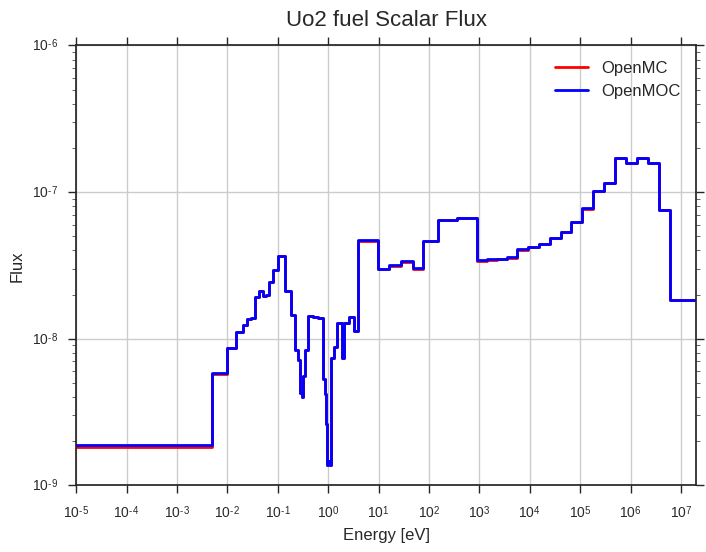
\includegraphics[width=0.9\linewidth]{figures/biases/pin-cell/flux-uo2-fuel}
  \caption{}
\label{fig:chap2-pin-flux}
\end{figure}

\begin{figure}
  \centering
  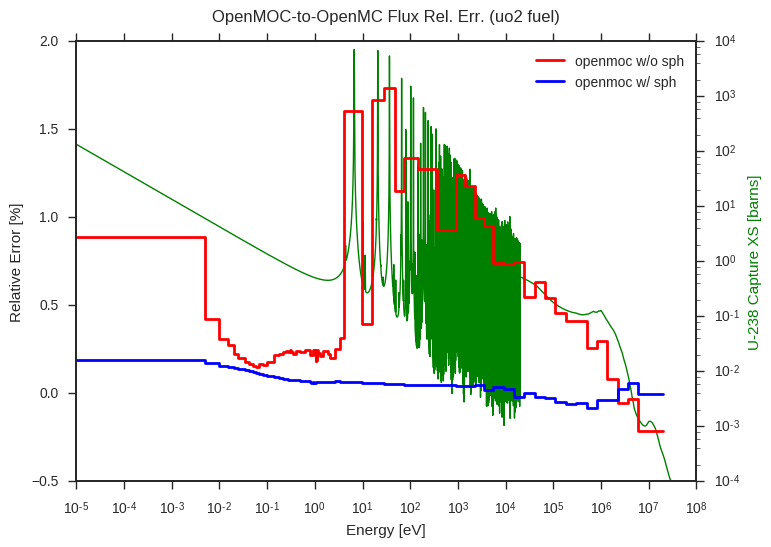
\includegraphics[width=0.9\linewidth]{figures/biases/pin-cell/rel-err-uo2-fuel}
  \caption{}
\label{fig:chap2-pin-flux}
\end{figure}


%%%%%%%%%%%%%%%%%%%%%%%%%%%%%%%%%%%%%%%%%%%
\subsection{2D Heterogeneous Fuel Assembly}

%%%%%%%%%%%%%%%%%%%%%%%%%%%%%%%%%%%%
\subsubsection{Track Discretization}
\label{subsubsec:chap4-hetero-lattice-tracks}

\begin{itemize}[noitemsep]
  \item plot of eigenvalue bias vs. azimuthal angle - curves for different track spacings
\end{itemize}

%%%%%%%%%%%%%%%%%%%%%%%%%%%%%
\subsubsection{Energy Groups}
\label{subsubsec:chap4-hetero-lattice-energy}

\begin{itemize}[noitemsep]
  \item table of eigenvalue bias by \# groups
\end{itemize}
